\chapterimage{img/comb.jpg} 
\chapter{Combination of Functions}
\section{Arithmetic Combinations of Functions}
Just as two real numbers can be combined by the operations of addition, subtraction, multiplication, and division to form other real numbers, two functions can be combined to create new functions. For example, the functions given by $f(x)=2x-3$ and $g(x)=x^2-1$ can be combined to form the sum, difference, product, and quotient of $f$ and $g$. \cite{ci}

\begin{align*}
    f(x)+g(x)   &=  (2x-3)+(x^2-1)\\
                &=  x^2+2x+4        &&\text{Sum}\\
    f(x)-g(x)   &=  (2x-3)-(x^2-1)\\
                &=  -x^2+2x-2       &&\text{Difference}\\
    f(x)g(x)    &=  (2x-3)(x^2-1)\\
                &=  2x^3-3x^2-2x+3  &&\text{Product}\\
    \dfrac{f(x)}{g(x)}   &=  \dfrac{2x-3}{x^2-1}, \qquad x\neq \pm 1      &&\text{Quotient}
\end{align*}

The domain of an \textbf{arithmetic combination} of functions $f$ and $g$ consists of all real numbers that are common to the domains of $f$ and $g$. In the case of the quotient $\dfrac{f(x)}{g(x)}$, there is the further restriction that $g(x)\neq 0$. \cite{ci}

\begin{example}[Finding the Sum of Two Functions] \cite{ci}~\\
    Given $f(x)=2x+1$ and $g(x)=x^2+2x-1$, find $(f+g)(x)$. Then evaluate the sum when $x=3$.\\
    \begin{solution}
        $$(f+g)(x) = f(x)+g(x) = (2x+1) + (x^2+2x-1) = x^2+4x$$
        When $x = 3$, the value of this sum is
        $$(f+g)(3) = (3)^2+4(3)  =21.$$
    \end{solution}
\end{example}
\begin{example}[Finding the Difference of Two Functions] \cite{ci}~\\
    Given $f(x)=2x+1$ and $g(x)=x^2+2x-1$, find $(f-g)(x)$. Then evaluate the sum when $x=2$.\\
    \begin{solution}
        $$(f-g)(x) = f(x)-g(x) = (2x+1) - (x^2+2x-1) = -x^2+2$$
        When $x = 2$, the value of this sum is
        $$(f-g)(3) = -(2)^2+2  =-1.$$
    \end{solution}
\end{example}
\begin{example}[Finding the Product of Two Functions] \cite{ci}~\\
    Given $f(x)=x^2$ and $g(x)=x-3$, find $(fg)(x)$. Then evaluate the sum when $x=4$.\\
    \begin{solution}
        $$(fg)(x) = f(x)g(x) = (x^2)(x-3) = x^3-3x^2$$
        When $x = 3$, the value of this sum is
        $$(fg)(4) = (4)^3-3(4)^2  =16.$$
    \end{solution}
\end{example}
\begin{example}[Finding the Quotients of Two Functions] \cite{ci}~\\
    Given $f(x)=\sqrt{x}$ and $g(x)=\sqrt{4-x^2}$, find $(f/g)(x)$ and $(g/f)(x)$. Then find the domains of $f/g$ and $g/f$\\
    \begin{solution}
        The quotient of $f$ and $g$ is
        $$\left(\dfrac{f}{g}\right)(x) = \dfrac{f(x)}{g(x)} = \dfrac{\sqrt{x}}{\sqrt{4-x^2}}$$
        and the quotient of $g$ and $f$ is 
        $$\left(\dfrac{g}{f}\right)(x) = \dfrac{g(x)}{f(x)} = \dfrac{\sqrt{4-x^2}}{\sqrt{x}}$$
        The domain of $f$ is $[0,\infty)$ and the domain of $g$ is $[2,-2]$. The intersection of these domains is $[0,2]$. So, the domains of $f/g$ and $g/f$ are as follows.
        $$\text{Domain of }\dfrac{f}{g}: [0,2) 
        \qquad
        \text{Domain of }\dfrac{g}{f}: (0,2] $$
    \end{solution}
\end{example}

\section{Composition of Functions}

\begin{definition}[Composition of Two Functions] 
    The \textbf{composition} of the function $f$ with the function $g$ is
    $$(f\circ g)(x)=f(g(x)).$$
    The domain of $f\circ g$ is the set of all $x$ in the domain of $g$ such that $g(x)$ is in the domain of $f$. (See Figure \ref{fig:domain_comp}.)
    \\\cite{ci}
\end{definition}

\begin{figure}[h]
\centering
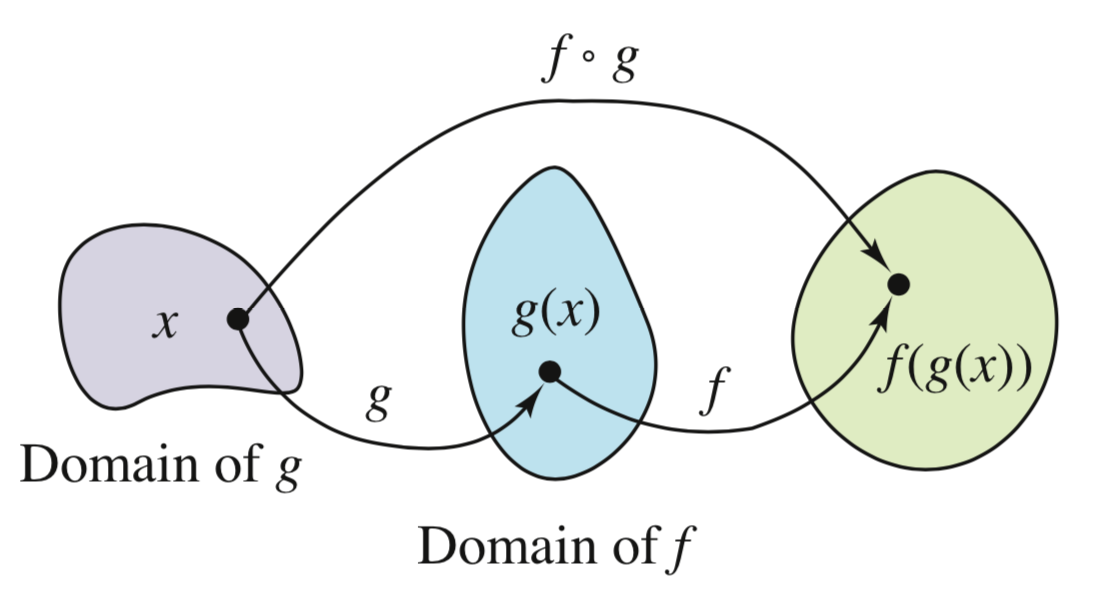
\includegraphics[scale=0.5]{img/fig/domain_comp.png}
\caption{Domain of a Composition Function \cite{ci}}
\label{fig:domain_comp}
\end{figure}

\begin{example}[Composition of Functions] \cite{ci}~\\
    Given $f(x)=x+2$ and $g(x)=4-x^2$, find the following.
    \begin{enumerate}
        \item $(f\circ g)(x)$ 
        \item $(g\circ f)(x)$
        \item $(g\circ f)(-2)$ 
    \end{enumerate}~\\
    \begin{solution}~\\
        \begin{enumerate}
            \item The composition of $f$ with $g$ is as follows.
            \begin{align*}
                (f\circ g)(x) &= f(g(x))\\
                &=f(4-x^2)
                &=(4-x^2)+2
                &=-x^2+6
            \end{align*}
            \item The composition of $g$ with $f$ is as follows.
            \begin{align*}
                (g\circ f)(x) &= g(f(x))\\
                &=g(x+2)
                &=4-(x+2)^2
                &=-x^2-4x
            \end{align*}
            Note that, in this case, $(f\circ g)(x)\neq (g\circ f)(x)$.
            \item Using the result of part 2, you can write the following.
            \begin{align*}
                (g\circ f)(-2) &=-(-2)^2-4(-2)
                &= -4+8
                &= 4
            \end{align*}
        \end{enumerate}
    \end{solution}
\end{example}

\section{Application}

\begin{example}[Bacteria Count] \cite{ci}~\\
    The number $N$ of bacteria in a refrigerated food is given by
    $$N(T)=20T^2-80T+500, \qquad 2\leq T \leq 14$$
    where $T$ is the temperature of the food in degrees Celsius. When the food is removed from refrigeration, the temperature of the food is given by
    $$T(t)=4t+2, \qquad 0\leq t\leq 3$$
    where $t$ is the time in hours.
    \begin{enumerate}
        \item Find the composition $N(T(t))$ and interpret its meaning in context.
        \item Find the time when the bacteria count reaches 2000.
    \end{enumerate}
    ~\\
    \begin{solution}~\\
        \begin{enumerate}
            \Item \begin{align*}
                N(T(t)) 
                &= 20(4t+2)^2-80(4t+2)+500\\
                &= 20(16t^2+16t+4)-320t-160+500\\
                &= 320t^2+320t+80-320t-160+500\\
                &= 320t^2+420
            \end{align*}
            The composite function $N(T(t))$ represents the number of bacteria in the food as a function of the amount of time the food has been out of refrigeration.
            \item The bacteria count will reach 2000 when $320t^2+420=2000$. Solve this equation for $t$ as shown.
            \begin{align*}
                320t^2+420 &= 2000\\
                320t^2 &= 1580\\
                t^2 &= \dfrac{79}{16}\\
                t &= \dfrac{\sqrt{79}}{4}\\
                t &\approx 2.2
            \end{align*}
            So, the count will reach 2000 when $t\approx 2.2$ hours.
            When you solve this equation, note that the negative value is rejected because it is not in the domain of the composite function.
        \end{enumerate}
    \end{solution}
\end{example}

\begin{exercise}
    ~\\\-\hspace{0.3cm} \textbf{
        In Exercises 1–2, find (a) $(f+g)(x)$, (b) $(f-g)(x)$, (c) $(fg)(x)$, and (d) $(f/g)(x)$.
    }\cite{ci}\\
    \begin{enumerate} 
		\item $f(x) = x^2,\quad g(x)=4x-5$
		\item $f(x) = \dfrac{1}{x},\quad g(x)=\dfrac{1}{x^2}$
    \end{enumerate}
    ~\\\-\hspace{0.3cm} \textbf{
        In Exercises 3–5, evaluate the indicated function for
        $f(x)=x^2+1$ and $g(x)=x-4$.
    }\cite{ci}\\
    \begin{enumerate}
        \setcounter{enumi}{2}
        \item $(f+g)(2)$
        \item $(fg)(6)$
        \item $(f/g)(-1)-g(3)$
    \end{enumerate}
    % ~\\\-\hspace{0.3cm} \textbf{
    %     In Exercises 7–10, find any vertical and horizontal Asymptotes.
    % }\cite{ci}\\
    % \begin{enumerate}
    %     \setcounter{enumi}{8}
    %     \item $f(x)=-\dfrac{1}{(x-2)^2}$
    %     \item $f(x) = \dfrac{2x^2-5x-3}{x^3-2x^2-5x+6}$
    %     \item $f(x) = \dfrac{5(x+4)}{x^2+x-12}$
    %     \item $f(x) = \dfrac{1-2x}{x}$
    % \end{enumerate}
\end{exercise}
